\chapter{Experiments and Results}
\label{AER}
This section presents the experimental results obtained from investigating the interactions between bacteria and phages under varying resource levels. 
We first describe bacterial growth in the absence of phages across resource conditions to establish a baseline. 
Next, we report the effects of phage exposure on bacterial survival. 
Finally, we examine phage population changes over time. 
Data are presented as means ± standard deviations and supported by appropriate statistical analyses.

\section{Graph Behavior}
\Cref{tab:results:graph_behavior} elaborates how a change in parameter value changes the shape and population level of the agents. 
\Cref{fig:created:a_good_curve_linear} is used as the reference graph to compare the graphs. 
The default values for \Cref{fig:created:a_good_curve_linear} can be found in \Cref{tab:appendixE:a_good_curve}.  
Each parameter was individually changed to a higher and lower value from the reference value, and the changes are noted in \Cref{tab:results:graph_behavior}. 

\begin{table}
    \small 
    \centering
    \begin{tabularx}{\textwidth}{l l X}
        \toprule
        \textbf{Parameter} & \textbf{Tested Value} & \textbf{Description of Behavior} \\
        \midrule
        $R$ (400) & 500 & More uninfected and infected, slightly more phages.\\
         & 300 & Slightly less uninfected and infected, earlier resource depletion.\\

        \midrule
        $U$ (50) & 70 & Slightly more phages and uninfected and infected bacteria.\\
         & 30 & Less uninfected and infected bacteria, slower resource depletion, not all resources used, slightly less phages. \\

        \midrule
        $P$ (10) & 20 & Less resources consumed, less uninfected, bacteria peaks earlier, slightly less phages.\\
         & 5 & Resources consumed faster, more uninfected, infected, and phages.\\

        \midrule
        $\tau$ (2.14) & 10 & Faster resource depletion, faster bacteria peak, plateau, then fall in population. more uninfected and infected, less phages.\\
         & 0.5& Barely any resource consumption, little bacteria growth and uninfected, more phages.\\

        \midrule
        $\omega^i$ (0) & 15 & Slightly more bacteria, resource replenish after bacteria die out.\\

        \midrule
        $e$ (0.03) & 0.1 & Faster resource depletion, sharper decline in uninfected, less infected and phages. \\
         & 0.01 & Less resource consumption, slightly more bacteria.\\

        \midrule
        $v$ (1.2) & 1.8 & More phages, significantly more bacteria, earlier and sharp peak in uninfected. \\
         & 1 & Less phages and bacteria, less resource consumption, earlier bacteria peak.\\

        \midrule
        $K$ (10) & 100 & Less resource consumption, less bacteria and phages, earlier bacteria peak.\\
         & 1 & Faster resource depletion and sudden stop instead of gradual slowdown, earlier bacteria peak.\\

        \midrule
        $r$ (0.01) & 0.1 & Less consumption, less infected and phages, earlier peak in bacteria..\\
         & 0.001 & Faster resource consumption rate, more infected and phages, delay in bacteria peak, sharp bacteria peak, small plateau in bacteria count before drop.\\

        \midrule
        $\beta$ (20) & 50 & More phages, earlier bacteria peak, less resources consumed, less bacteria.\\
         & 10 & Faster resource consumption, more uninfected, less phages, sharper bacteria peak.\\

        \midrule
        $\omega^o$ (0) & 0.02 & Faster resource depletion, more bacteria and sharper peak, later peak, and less phages. \\

        \bottomrule
    \end{tabularx}
    \caption{
        A table that compares how moving one individual parameter value up or down relative to \Cref{fig:created:a_good_curve_linear} changes the general shape of the curve. 
        This table is not meant to be exhaustive, cover edge cases, or extreme cases, or cover every exact detail and change in the population graph, but just to give an idea of how a change in parameter influences the graph shape, such as the rate of resource depletion, maximum number of bacteria and phages, and change in peak time. 
        Reference parameter values used to compare the produced curves are included in the parentheses, taken from \Cref{tab:appendixE:a_good_curve}. 
    }
    \label{tab:results:graph_behavior}
\end{table}

\section{SOBOL Sensitivity Analysis Results}
\label{sec:SOBOL_sensitivity_analysis_results}

\Cref{fig:created:SOBOL_final} shows the impact that the parameter had on the final value of the population at $t=15$. 
The average value and variance of population value were intentionally left out of the analysis, despite being a part of the dashboard because the SOBOL sensitivity values are almost identical to the final sensitivity values. 
It also doesn't make sense to measure the average and variance of the population given the dynamics of the system. 
Given the similarity among the plots, the analysis will focus on the final value as shown in \Cref{fig:created:SOBOL_final}.

The parameters that were tested include all the parameters listed in the extended golden model, except for Uninfected Bacteria and $M$. 
Uninfected Bacteria was left out as it doesn't make sense to already add infected bacteria to the system
$M$, the number of stages that the infection goes through, can not be tested as $M$ hardcodes the number of infection stages that the bacteria has to go through. 
The hardcoding is done before the simulation framework starts. 
As such, it is not possible to change $M$ without rerunning the program from the very start. 

\subsection{Final Value Analysis}
\subsubsection{Resources}
The washin rate and washout rate consistently had the largest influence on the final, peak value, and time of peak value, using the 95\% rule. 
Despite the resource consumption rate directly depends on $e, v$ and $K$, the parameters had very little influence on the final value as evidence by the ST and S1 bar being near 0. 
The resource population was mainly driven by the washin and washout value. 
The peak resources are driven completely by the washin rate. 
Not many interactions between two or more parameters were occurring. 

\subsubsection{Phages}
The most important factor for the final phage value is $r$, followed by $\beta$ and $\omega^o$. 
The other parameters had little to no effect on the final phage value. 

\subsubsection{Total Bacteria}
The sum of uninfected and infected bacteria depended heavily on higher order interactions as $ST_i \gg S1_i$. 
Although not shown, the bar plots for the total bacteria resembled that of the bar-plots for the uninfected bacteria, and less that of the infected bacteria. 

\begin{figure}[ht!]
    \centering
    \begin{subfigure}{0.32\linewidth}
        \centering
        \captionsetup{width=1\linewidth}
        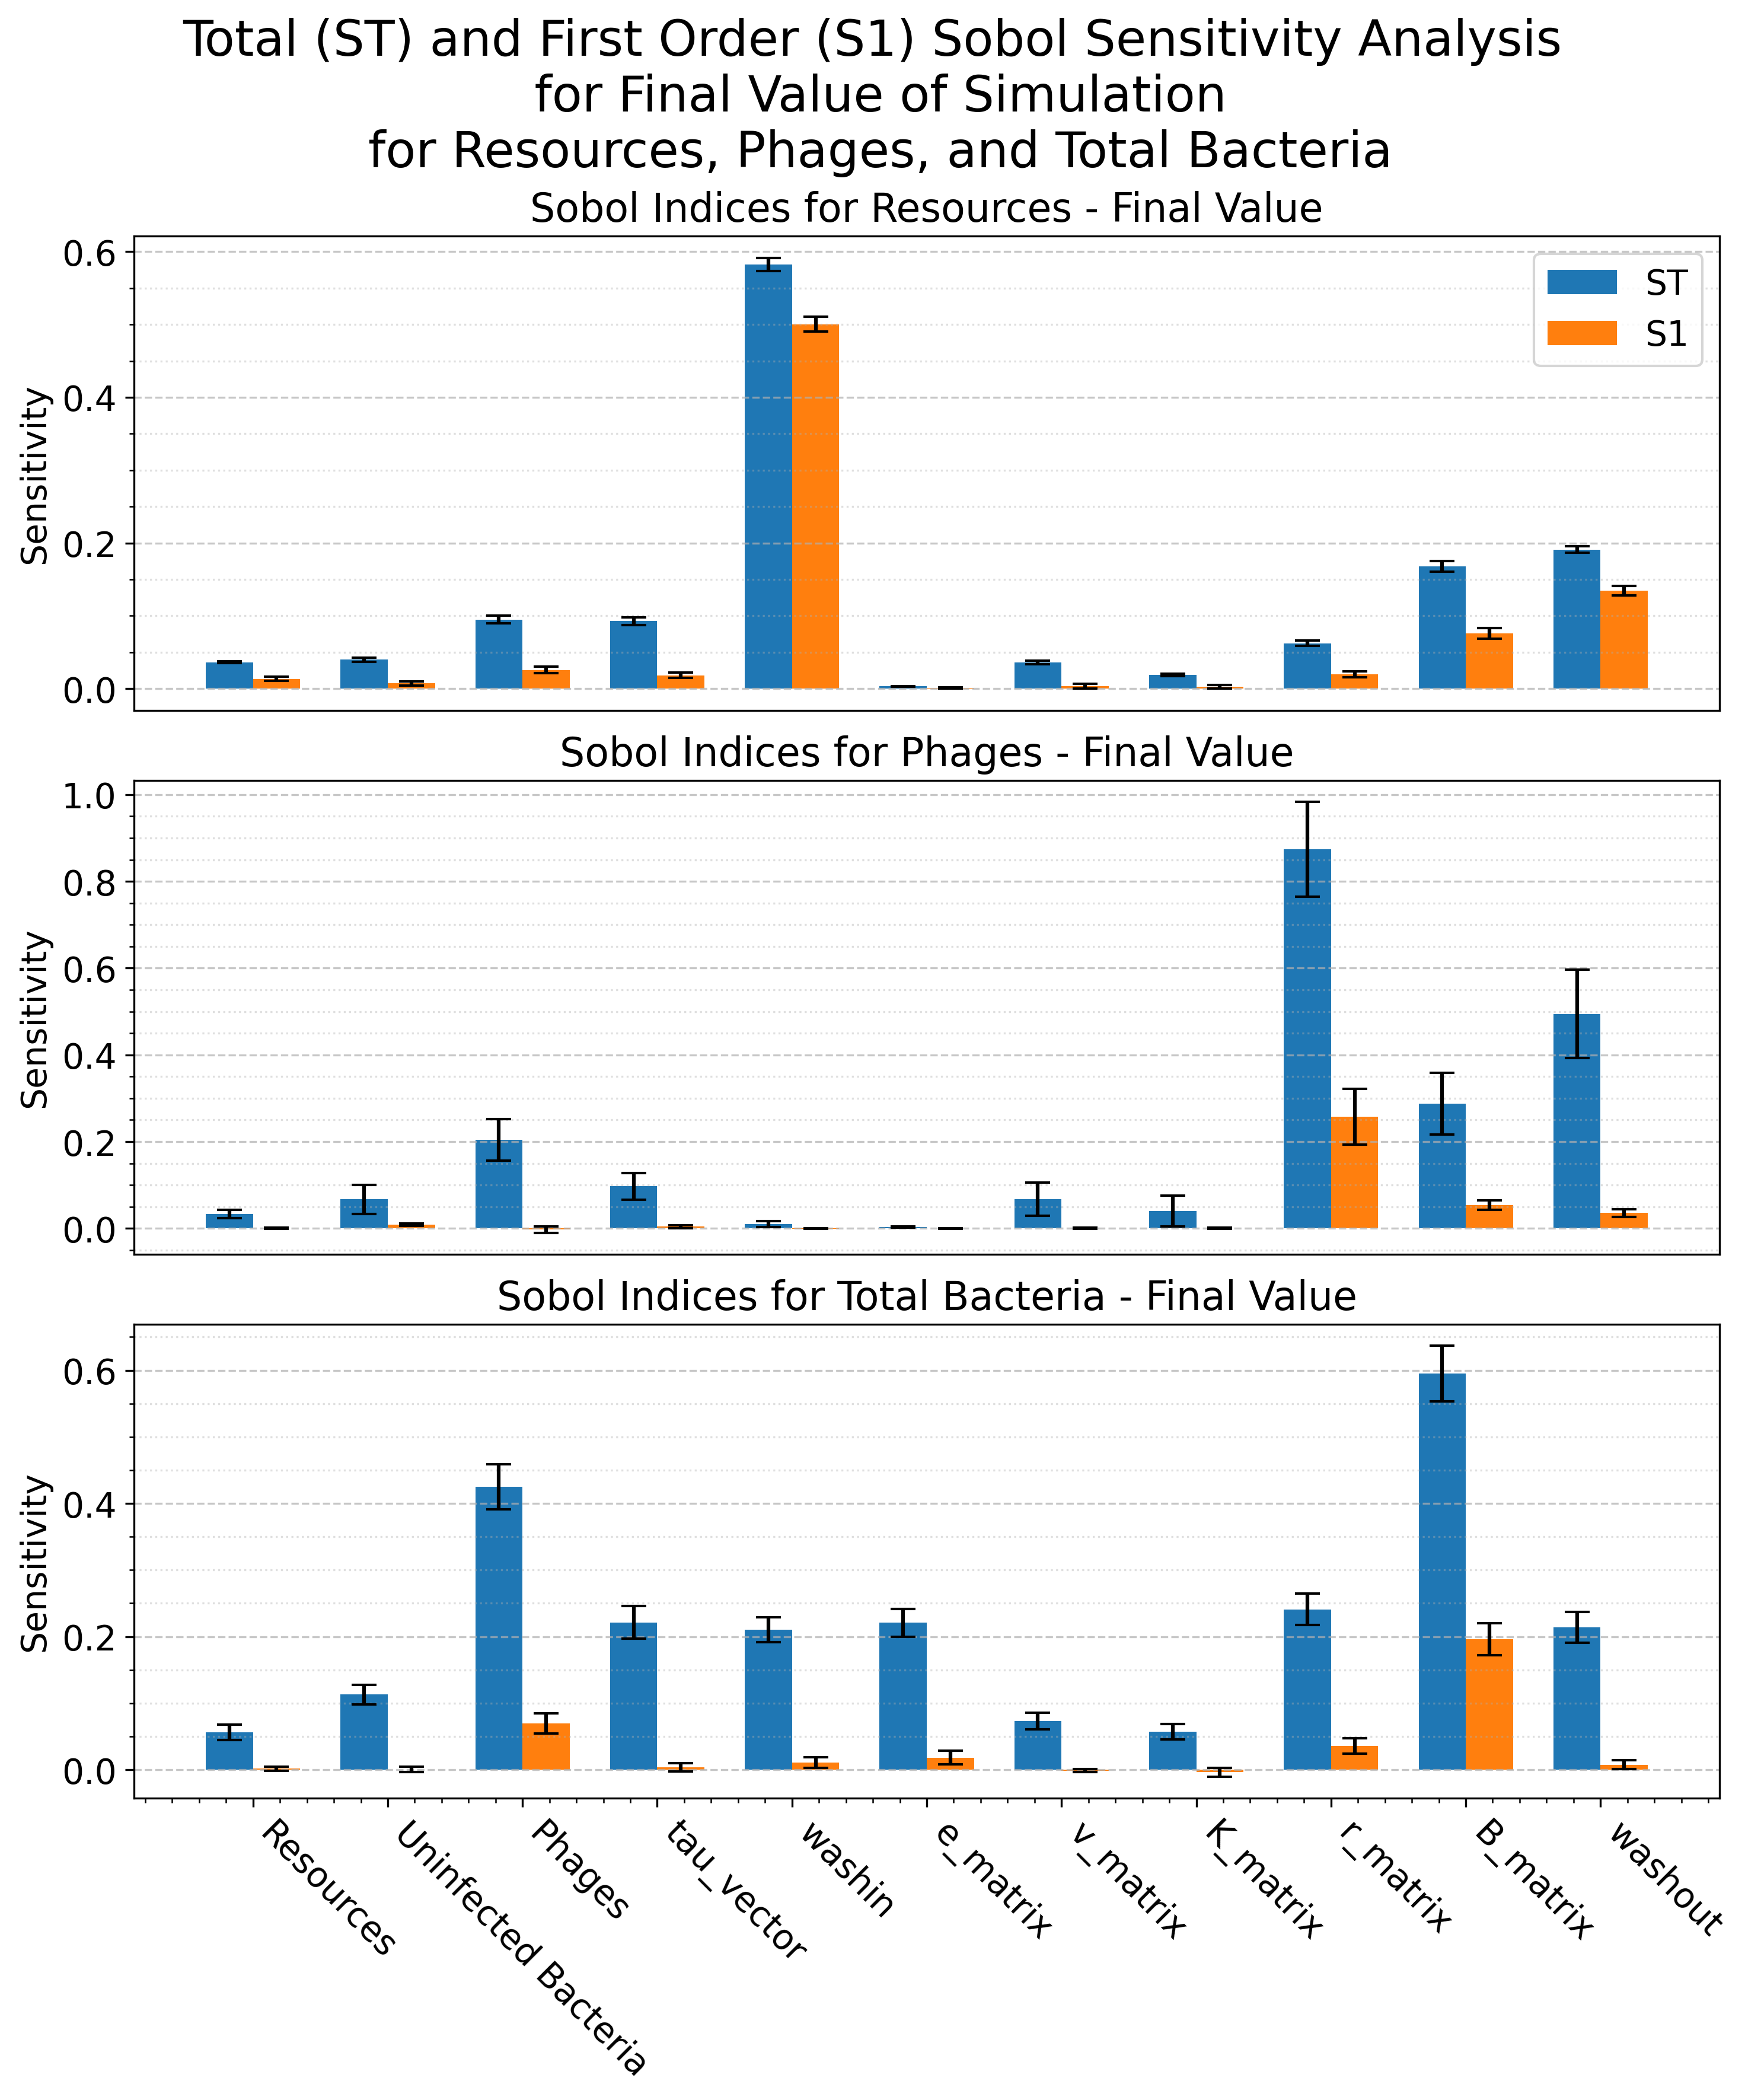
\includegraphics[width=\linewidth]{Plots/Created/SOBOL/SOBOL_analysis_1749149674_Final.png}
        \caption{
            Final population value. 
        }
        \label{fig:created:SOBOL_final}
    \end{subfigure}
    \hfill
    \begin{subfigure}{0.32\linewidth}
        \centering
        \captionsetup{width=1\linewidth}
        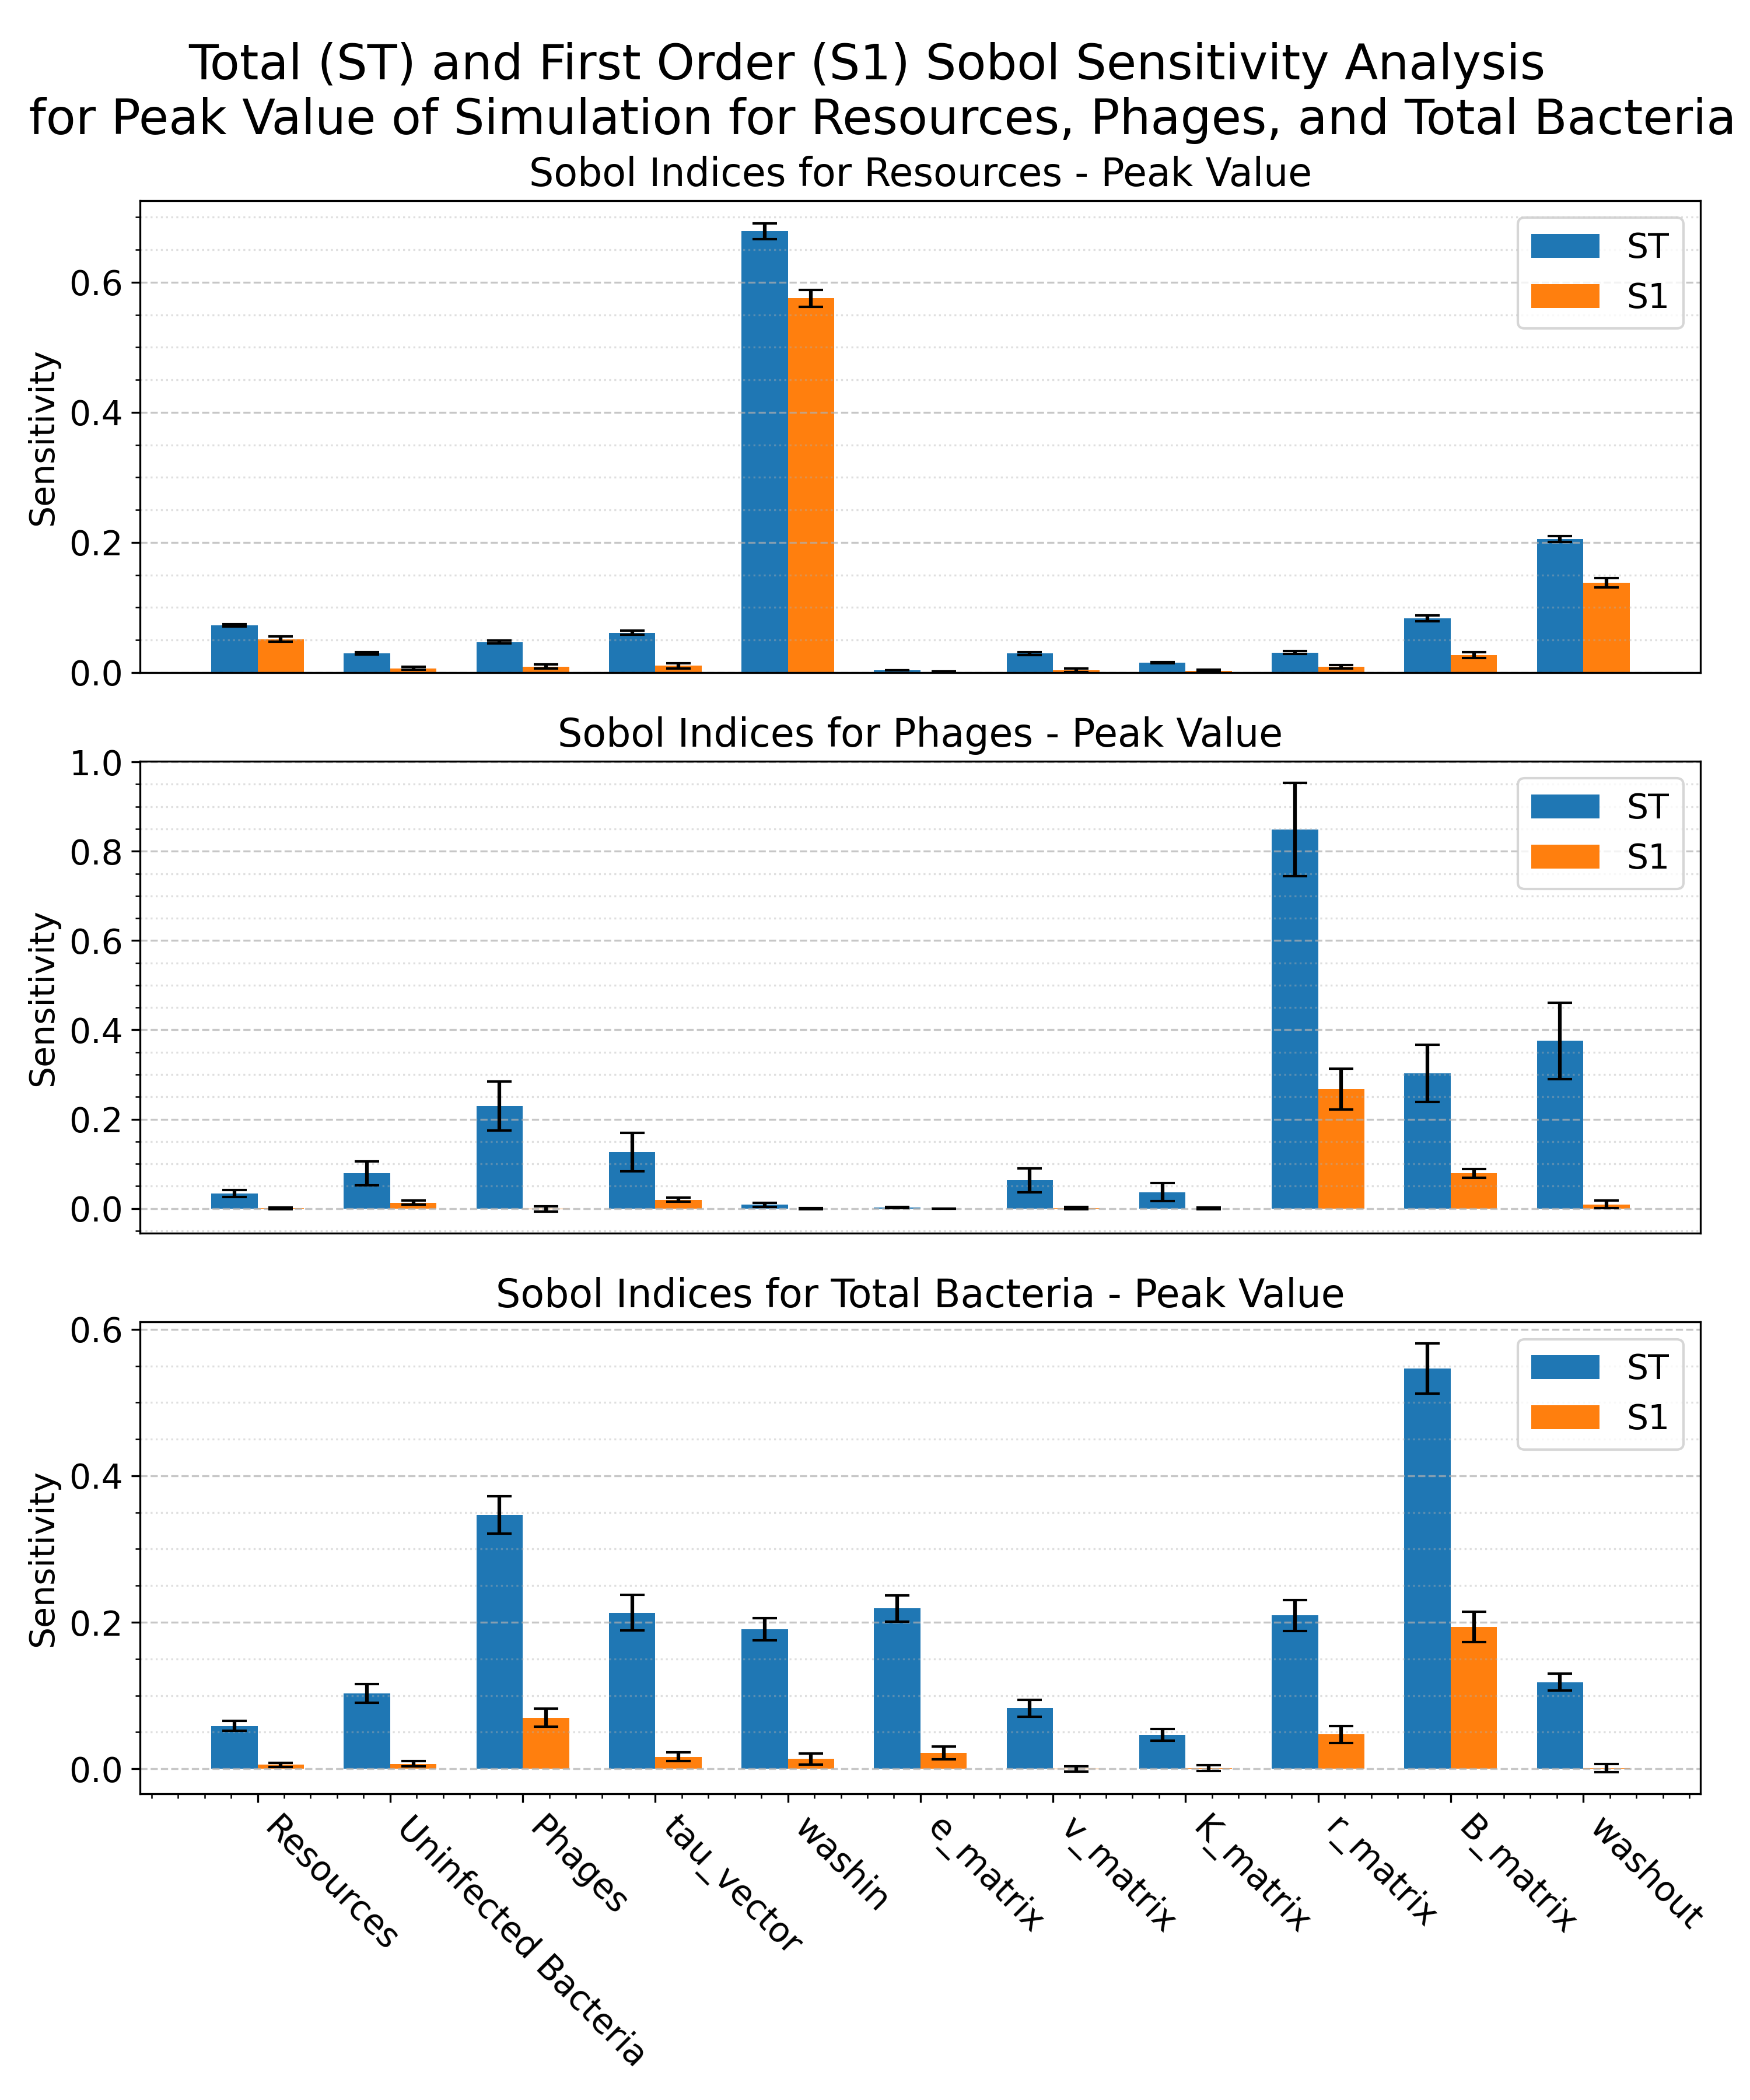
\includegraphics[width=\linewidth]{Plots/Created/SOBOL/SOBOL_analysis_1749149674_Peak.png}
        \caption{
            Peak population value. 
        }
        \label{fig:created:SOBOL_peak}
    \end{subfigure}
    \hfill
    \begin{subfigure}{0.32\linewidth}
        \centering
        \captionsetup{width=1\linewidth}
        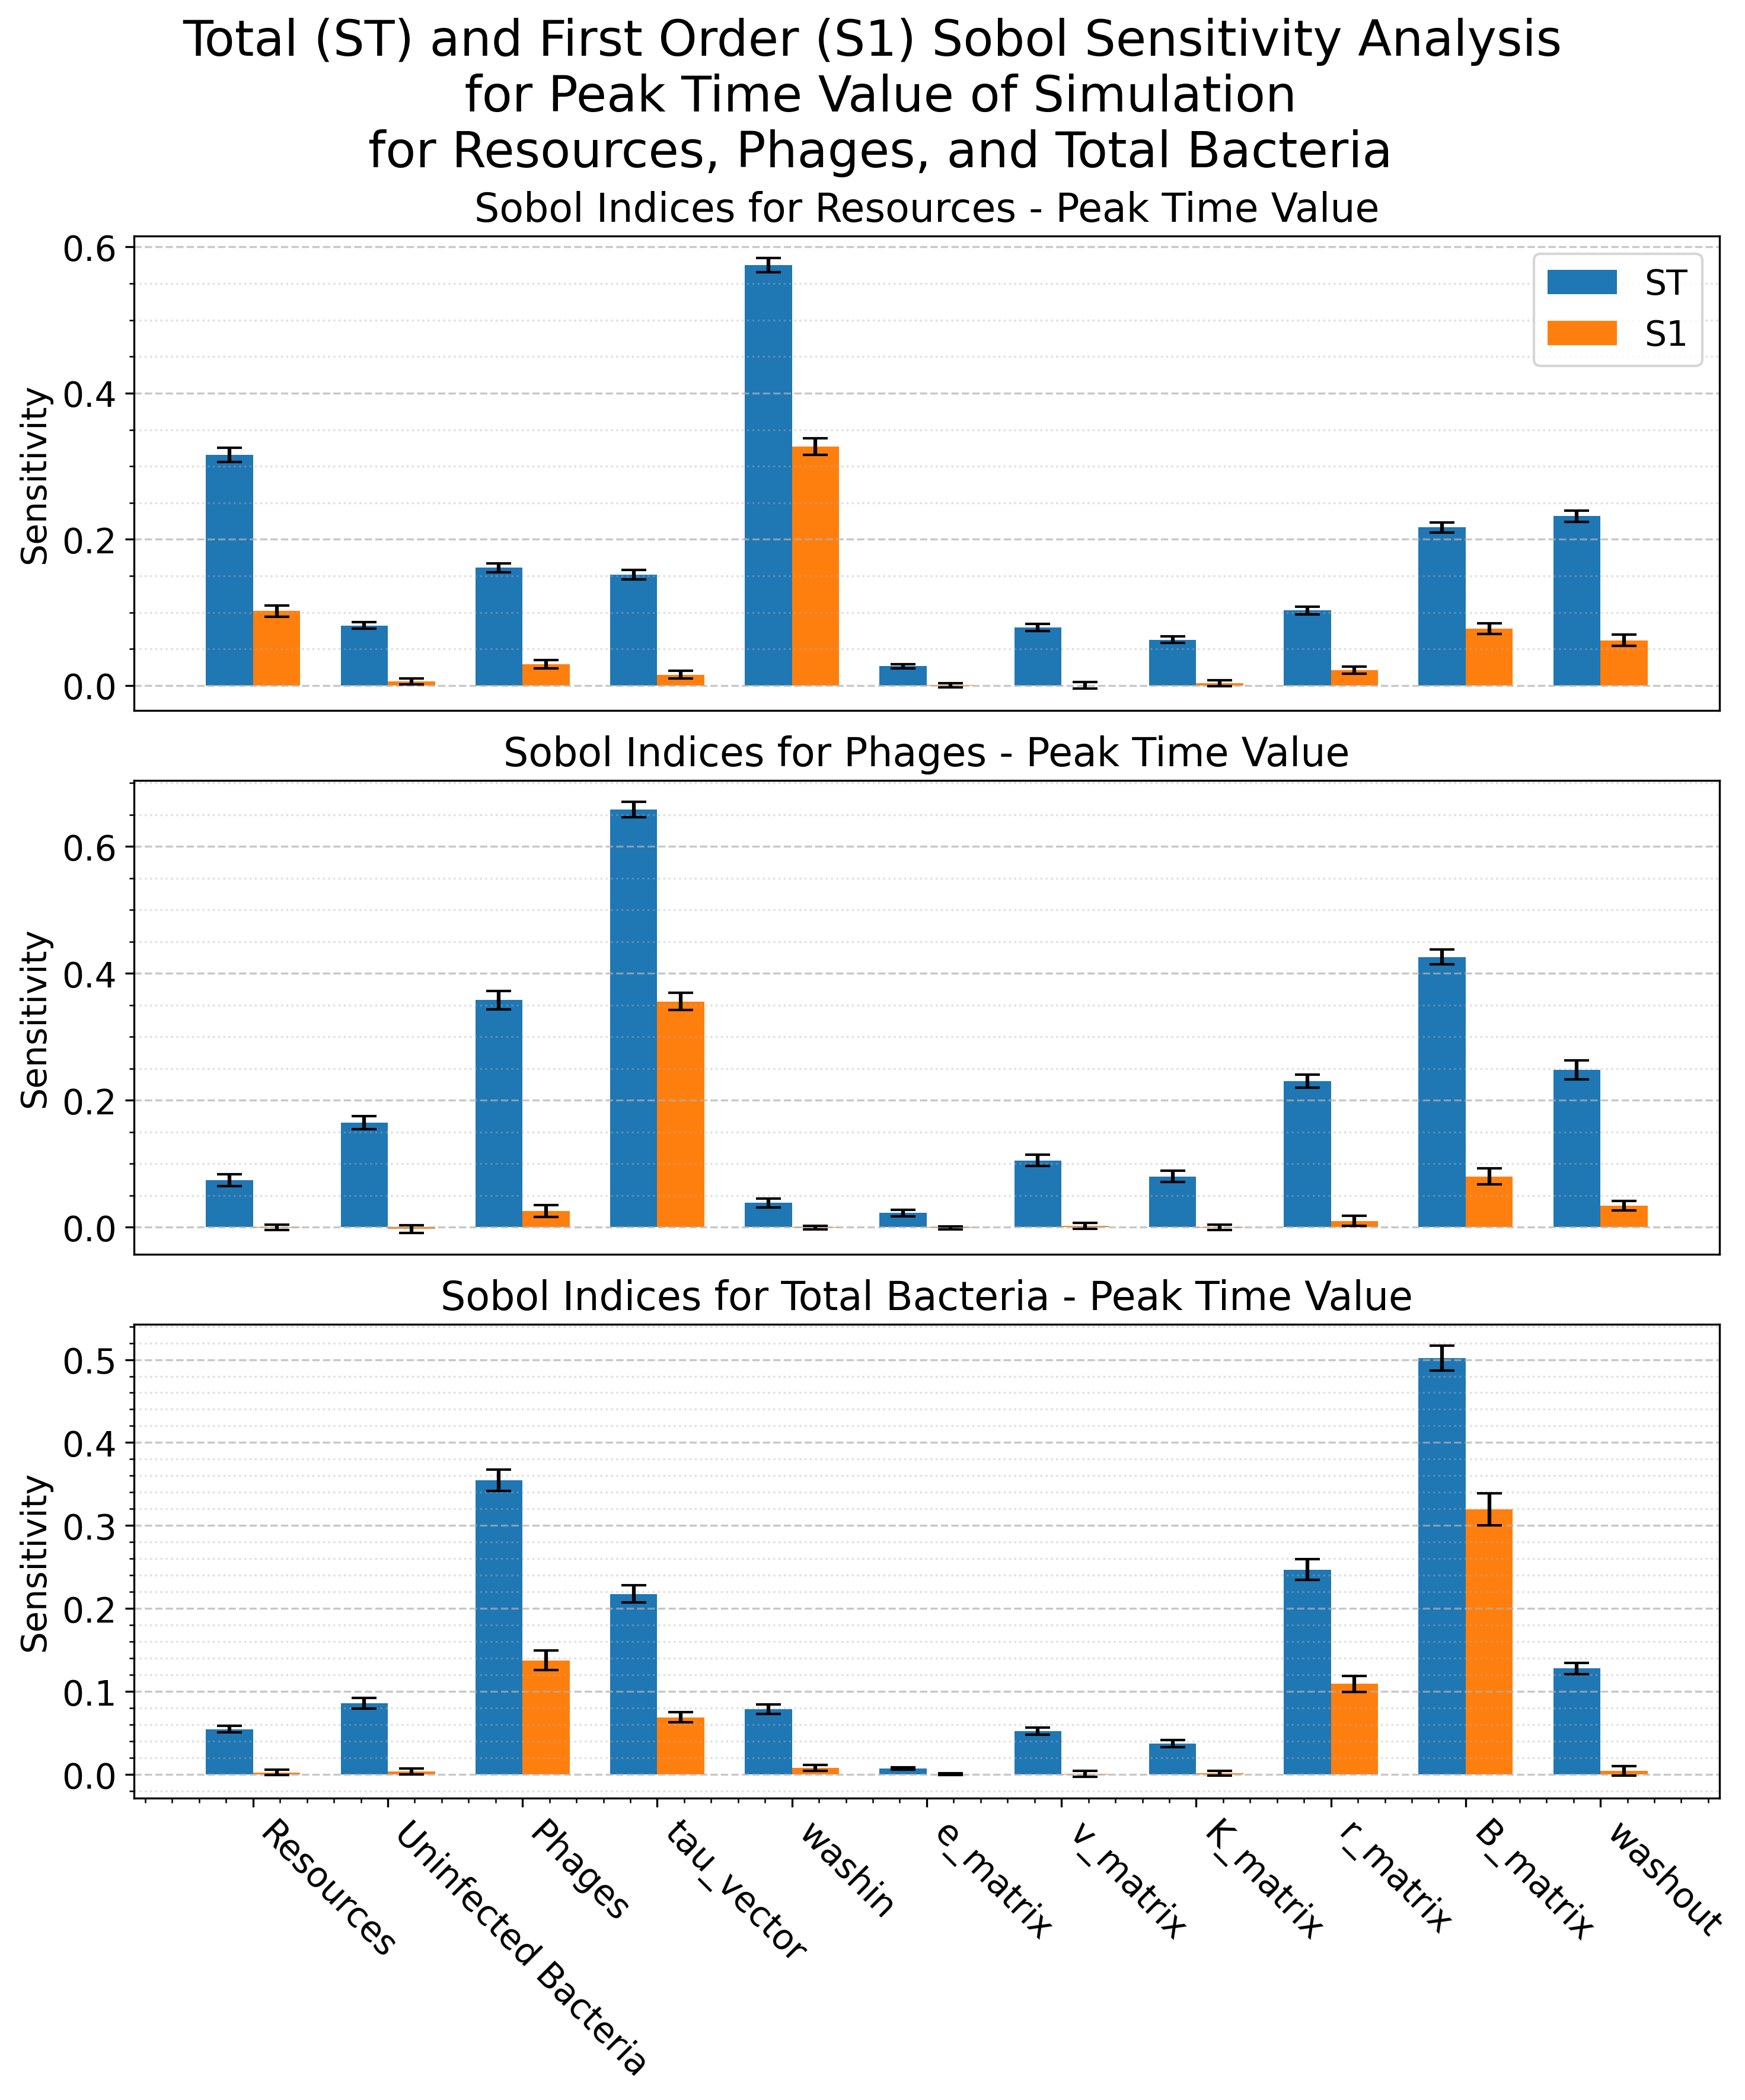
\includegraphics[width=\linewidth]{Plots/Created/SOBOL/SOBOL_analysis_1749149674_Peak_Time.png}
        \caption{
            Time at peak population. 
        }
        \label{fig:created:SOBOL_peak_time}
    \end{subfigure}
    \caption{
        SOBOL analyses for the final, peak, and time of peak value. 
        The data was saved from the dashboard and plotted using Matplotlib. 
        The values used for this SOBOL test can be found in \Cref{tab:appendixE:SOBOL_analysis_values}. 
        The data used in \Cref{fig:created:SOBOL_final} was used for \Cref{fig:created:SOBOL_peak} and \Cref{fig:created:SOBOL_peak_time}. 
    }
    \label{fig:created:SOBOL_analyses}
\end{figure}

\subsection{Custom SOBOL Analysis - Peak Value and Time of peak}
Due to the similarity of the final, average, and variance value as seen in \Cref{fig:created:SOBOL_final}, \Cref{fig:created:SOBOL_average_extra}, and \Cref{fig:created:SOBOL_variance_extra} a custom SOBOL analysis that isn't included in the dashboard might result in a different SOBOL analysis result. 
To create the custom SOBOL analyses, the peak value and the time at the peak of the population is measured and analyzed. 
The peak is defined as the point where the population reaches 95\% of its absolute maximum value. 
The time at peak is measured at the point in time that the population reaches 95\% of the maximum value. 
This removes unintended side effects of the simulation. 
For populations that are only increasing in value, this prevents the measured peak from bunching up at the end of the simulation, skewing the data. 
As the peak is defined at 95\% of the absolute maximum value, populations that have a faster increase on population count at the end will have a time value closer towards the end of the simulation. 
For populations that reach a plateau, the 95\% rule will push the peak time towards the beginning of the simulation, while still "respecting" the absolute final value since $95\% \approx 100\%$. 
The 95\% rule can fail under certain situations, such as when there is cyclic behavior. 
See \nameref{sec:appendixF:why_95} for a more detailed explanation on why the 95\% rule is used. 

The results of the SOBOL peak and time at peak analyses can be seen in \Cref{fig:created:SOBOL_peak} and \Cref{fig:created:SOBOL_peak_time}. 
Although some of the bars between the final, peak, and time at peak values are the same, some are different. 
But overall, similar values can be seen across the the final, peak, and time at peak analyses. 
The peak infected values are more certain compared to the final infected values, which could be due to the 95\% rule removing some of the noise of the simulation. 
The time at peak values have less error compared to the final and peak value. 
This is due to the restricted range of values. The time at peak value can only fall somewhere between 0 and 15, the start and end values of the simulation respectively. 
The final and peak values can fall anywhere between 0 and any value, depending on the IC and how high the population can rise, and how fast the population can fall, \textit{if} the population count falls. 

\subsection{SOBOL Analysis - Without Washin and Washout}
In many of the plots, the washin and washout rate had a large influence on the final, peak, and time of peak value. 
\Cref{fig:created:SOBOL_no_wi_wo_extra} ran the same input as \Cref{fig:created:SOBOL_analyses}, but left the washin and washout rate out. 
The sensitivity plots for the final, peak, and time of peak plots look different from one another. 
The final resource value depended heavily on the washin and washout rate, but without the washin and washout, the final resource depended heavily on the initial resource population. 
Since $S1 \approx ST$, the resource parameter does not depend on other higher order interactions. 

The peak value for the resources without washin and washout only depended on the initial resource consumption. 
Since there was no washin, no resources could be added, so the peak for the resources was always at $t=0$, and was dependent on the initial resource value. 
The time at peak value is always 0 as the resources are only being depleted, so no matter the change in parameter values, the parameter had no effect on the peak time, so SOBOL gives a value of 0 to every parameter for the resources. 
$\beta$ consistently had a large effect on the final, peak, and time of peak value. 


\section{Initial Value Analysis Results}
\label{sec:results:initial_value_analysis}

\Cref{fig:created:initial_value_analysis_UB_50_500_a_good_plot_2} and \Cref{fig:created:initial_value_analysis_UB_50_500_a_good_plot} illustrate how varying the initial uninfected bacteria population from 1 to 500 (using 100 different starting values) affects the dynamics and time of peak population of phage and total bacteria populations using the 95\% rule. 

\Cref{fig:created:initial_value_analysis_UB_50_500_a_good_plot_2} replicates  Figure 1 of \citet{mullaExtremeDiversityPhage2024} perfectly. 
As the initial bacteria population increases, the time to reach the phage and bacteria sum peak decreases, following $y = -0.8648\cdot ln(x) + 9.7911$ and $y = -1.0056\cdot ln(x)+7.7626$, with $R^2=0.9800, 0.9988$ respectively. 

\Cref{fig:created:initial_value_analysis_UB_50_500_a_good_plot} on the other hand shows different behavior. 
As the initial bacteria population decreases from 500 to 100, the same behavior in \Cref{fig:created:initial_value_analysis_UB_50_500_a_good_plot_2} is noticed.
However at 100 and less initial uninfected bacteria, there is a change in behavior. 
Instead of following the predicted line like in \Cref{fig:created:initial_value_analysis_UB_50_500_a_good_plot_2}, the curve for the phages suddenly decreases, following a quadratic like curve. 
The bacteria on the other hand plateau before starting to increase again. 
Both curves resemble a spoon-like shape. A straight handle with a "bowl" to hold the liquid. 
The fitted curves follow $y = -0.1292\cdot ln(x) + 10.1462$ and $y = -0.6234\cdot ln(x)+6.9602$, with $R^2=0.5406, 0.9206$ respectively. 
Despite the large bacteria sum $R^2$ value, the fitted curve does not fit the data. 

\begin{figure}
    \centering
    \begin{subfigure}{1\linewidth}
        \centering
        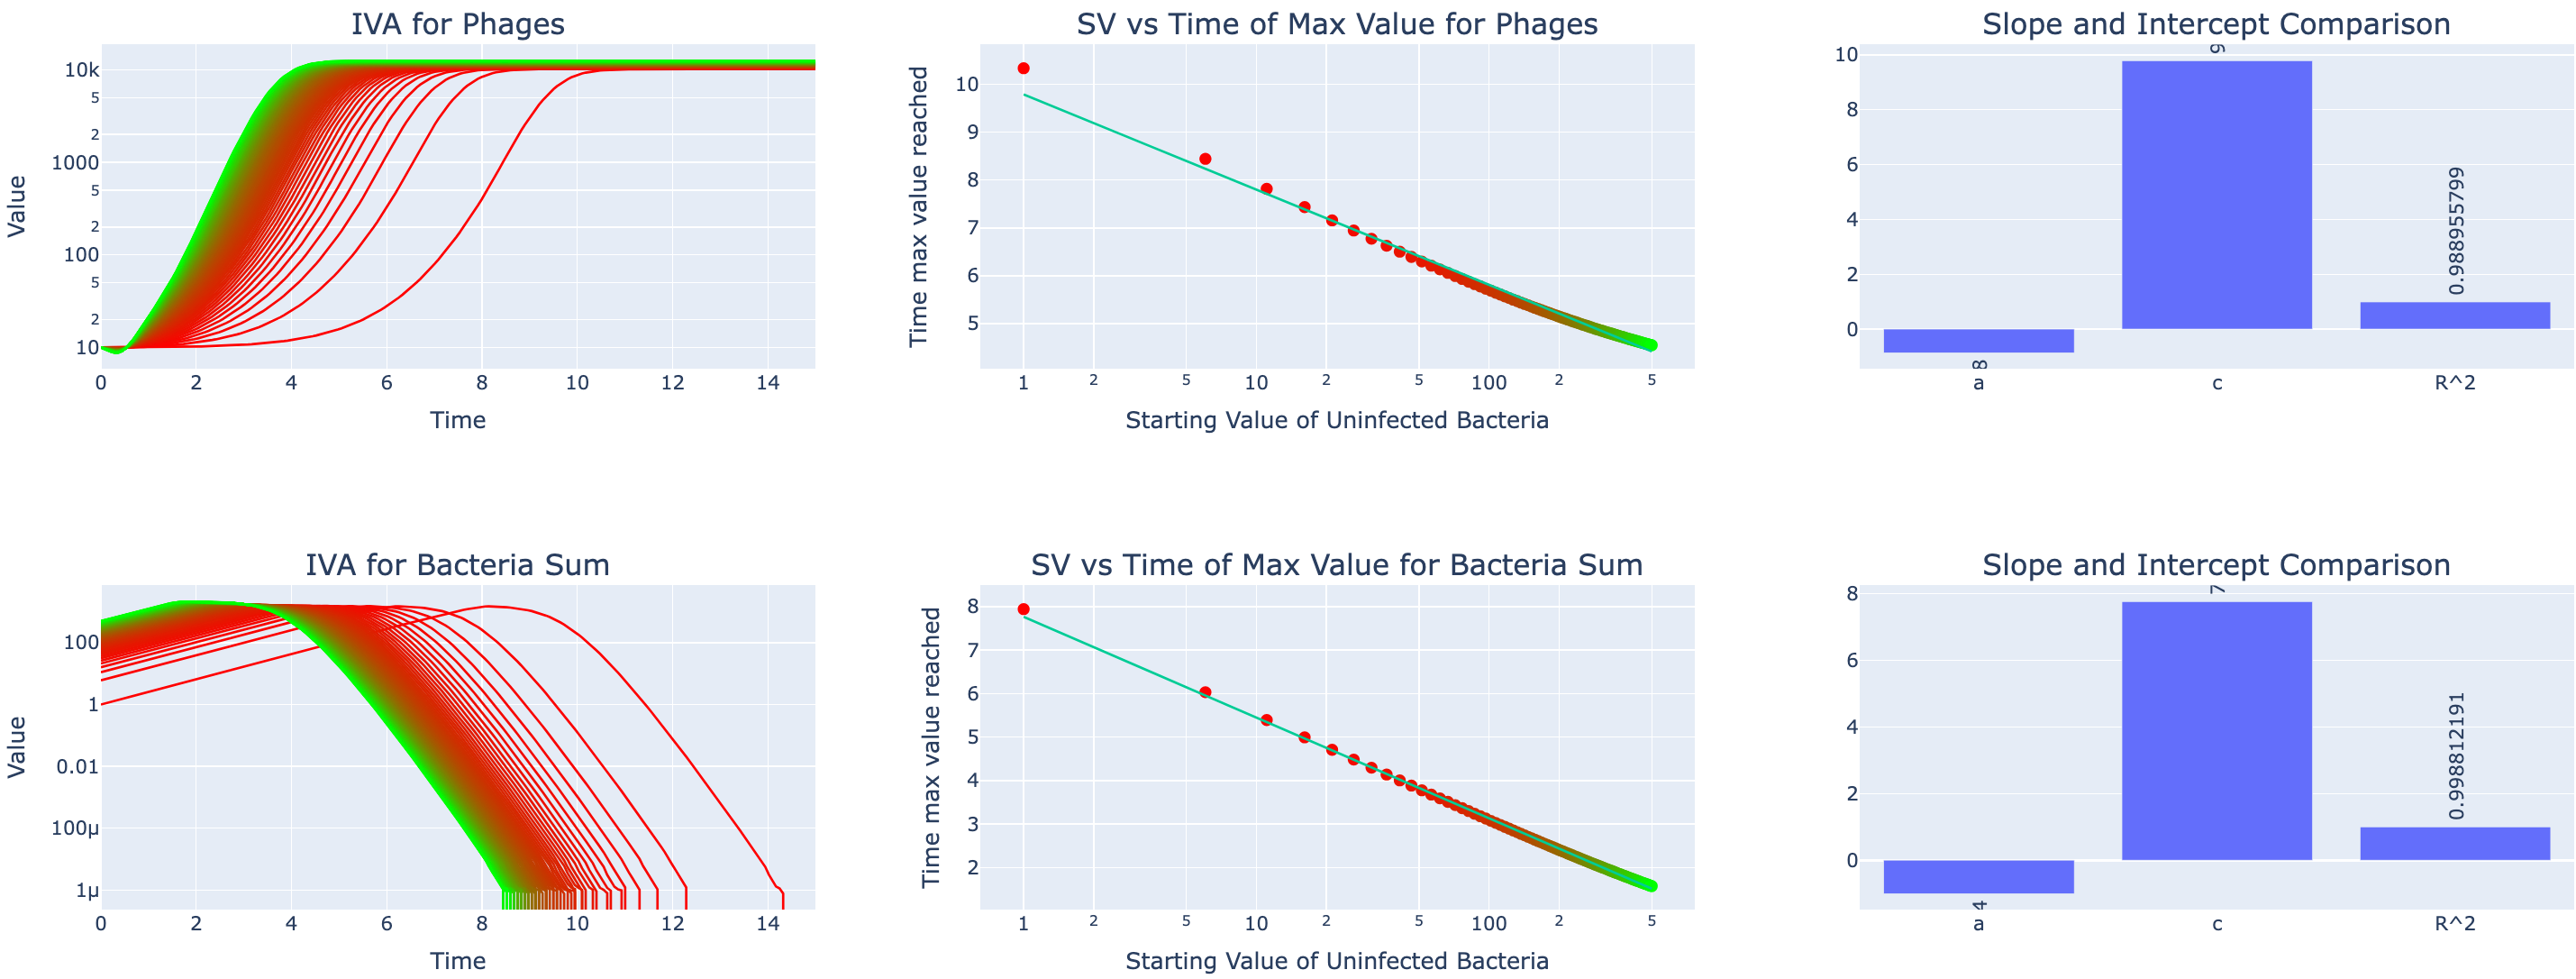
\includegraphics[width=\linewidth]{Plots/Created/IVA/initial_value_analysis_UB_50_500_a_good_plot_2.png}
        \caption{
            IVA for \Cref{tab:appendixE:a_good_curve_2}. 
            Replicates Figure 1 of \citet{mullaExtremeDiversityPhage2024}. 
        }
        \label{fig:created:initial_value_analysis_UB_50_500_a_good_plot_2}
    \end{subfigure}
    \hfill
    \begin{subfigure}{1\linewidth}
        \centering
        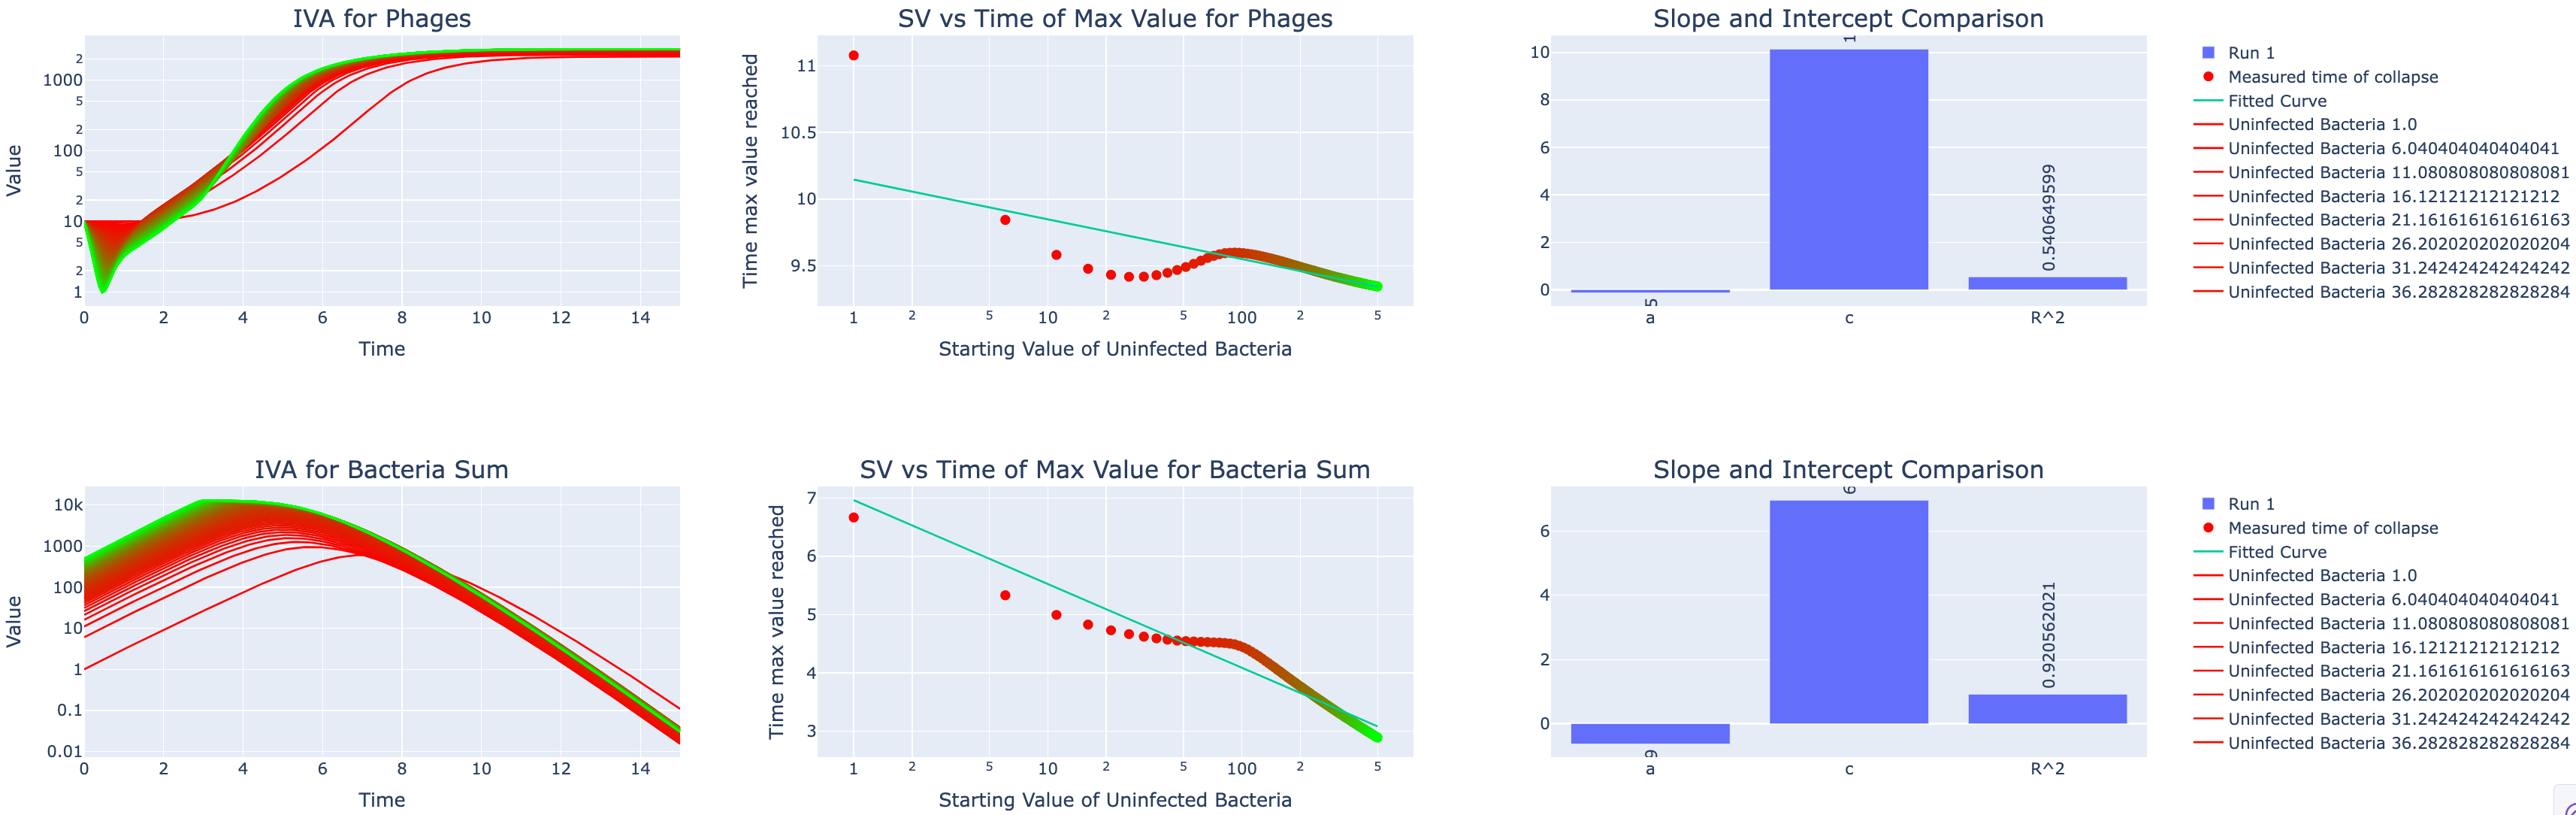
\includegraphics[width=\linewidth]{Plots/Created/IVA/initial_value_analysis_UB_50_500_a_good_plot.png}
        \caption{
            IVA for \Cref{tab:appendixE:a_good_curve}. 
            For uninfected bacteria less than 100, the phage-bacteria interaction is resource limited. 
        }
        \label{fig:created:initial_value_analysis_UB_50_500_a_good_plot}
    \end{subfigure}
    \caption{
        Varying initial Uninfected Bacteria concentration, from 50 to 500, with 30 unique values tested over two different instances of "good" curves. 
        Even with two "good" curves, even varying the default parameter values a tiny bit can have a large influence on how changing the initial bacteria concentration can have an influence on the dynamics of the system, changing the behavior of the peak time. 
        The default values for Figure a) and b) can be found at \Cref{tab:appendixE:a_good_curve} and \Cref{tab:appendixE:a_good_curve_2}. 
    }
\end{figure}


\section{Phase Portrait}
\label{sec:results:phase_portrait}
\Cref{fig:created:phase_portrait_resources_245-265_phages_25-26} shows a phase portrait varying the initial resource and phage concentration. 
For phages that start above 25.98, the phage population can proliferate (until the washout would eventually remove the phages). 
For phage populations that start below 25.98, the washout removes the phages before the phages had time to infect and kill the bacteria. 
Both regions of phages exhibit consistent behavior, of either going to 0 or proliferating. 
If the phage population started at exactly 25.98, if the initial resources was 260 or above, the phages died out. 
If the initial resources was 255 or below, the phages would proliferate. 
Expanding on these results by simulating more initial values creates \Cref{fig:created:phase_portrait_resources_phage}. 
The initial resource values span from 1 to 500, and the initial phage values range from 25.5 to 26.5, each with 100 unique values sampled.
Each cell is a unique set of initial conditions. 
If the phages proliferated for that condition, the box is colored red. 
In this case, proliferated means that the phage population reached at least 2 times the initial condition. 
If the box is white, it means  the phages died out before being able to reach 2 times its initial concentration. 
A boundary between the dead and proliferating phages can be curve-fit following $y=\frac{86.756x}{15.811+x} - 10.241$ with an $R^2$ value of 0.994. 
\Cref{fig:created:phase_portrait_resource_phage_proliferate} zooms into the range $(1-40, 24.2-25)$ for a high detailed view of the behavior happening around initial resources of 10. 
At about resources of 6 or 7, there is a minimum in phage proliferation. 
For initial resource values of 6 or below, as initial resources increase, less phages (although very miniscule changes) are required to proliferate. 
For initial resource values of 7 or above, more phages (although very miniscule changes) are required to proliferate. 

\begin{figure}[]
    \centering
    \begin{subfigure}{0.49\linewidth}
        \centering
        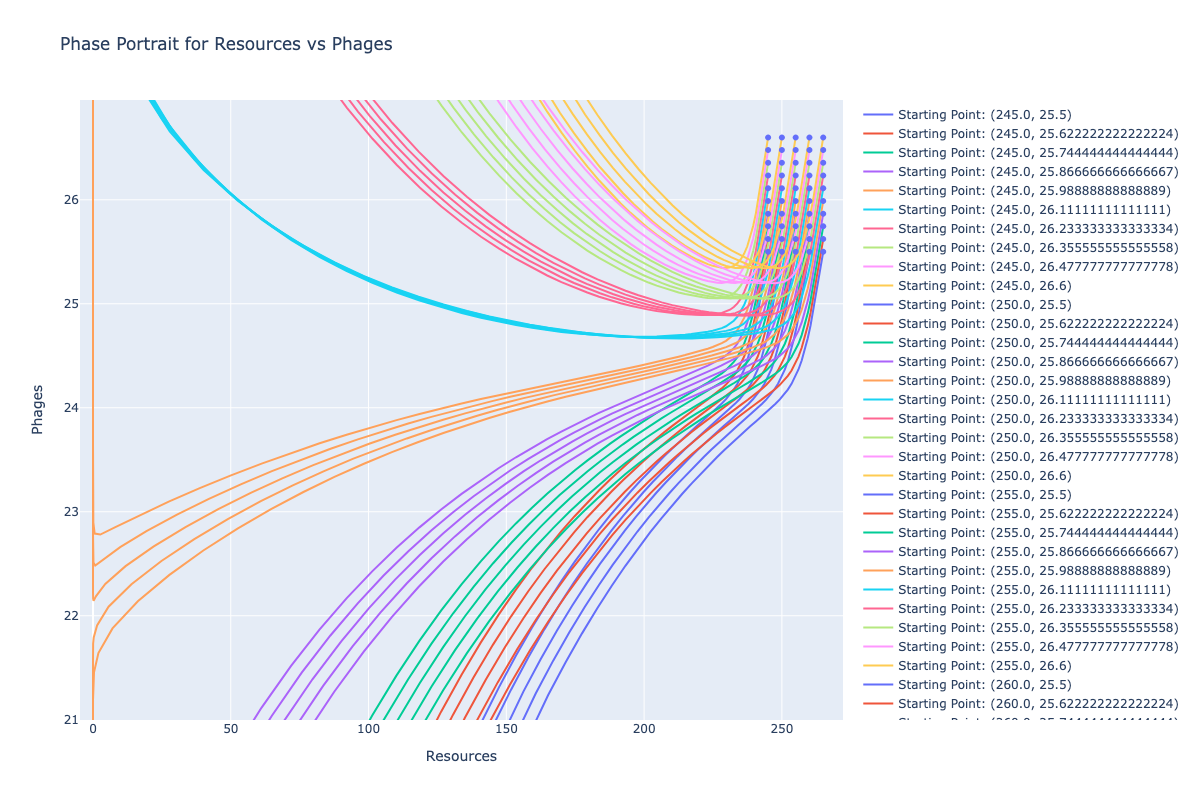
\includegraphics[width=1\textwidth]{Plots/Created/PP/phase_portrait_resources_245-265_phages_25-26.png}
        \caption{
            Zoomed in plot of a phase portrait with varying resource and phage population from 245-265 and 25.5-26.5 respectively. 
            Each row has its own line color. 
            Diverging behavior can be seen for the orange line (phage=25.98). 
        }
        \label{fig:created:phase_portrait_resources_245-265_phages_25-26}
    \end{subfigure}
    \hfill
    \begin{subfigure}{0.49\linewidth}
        \centering
        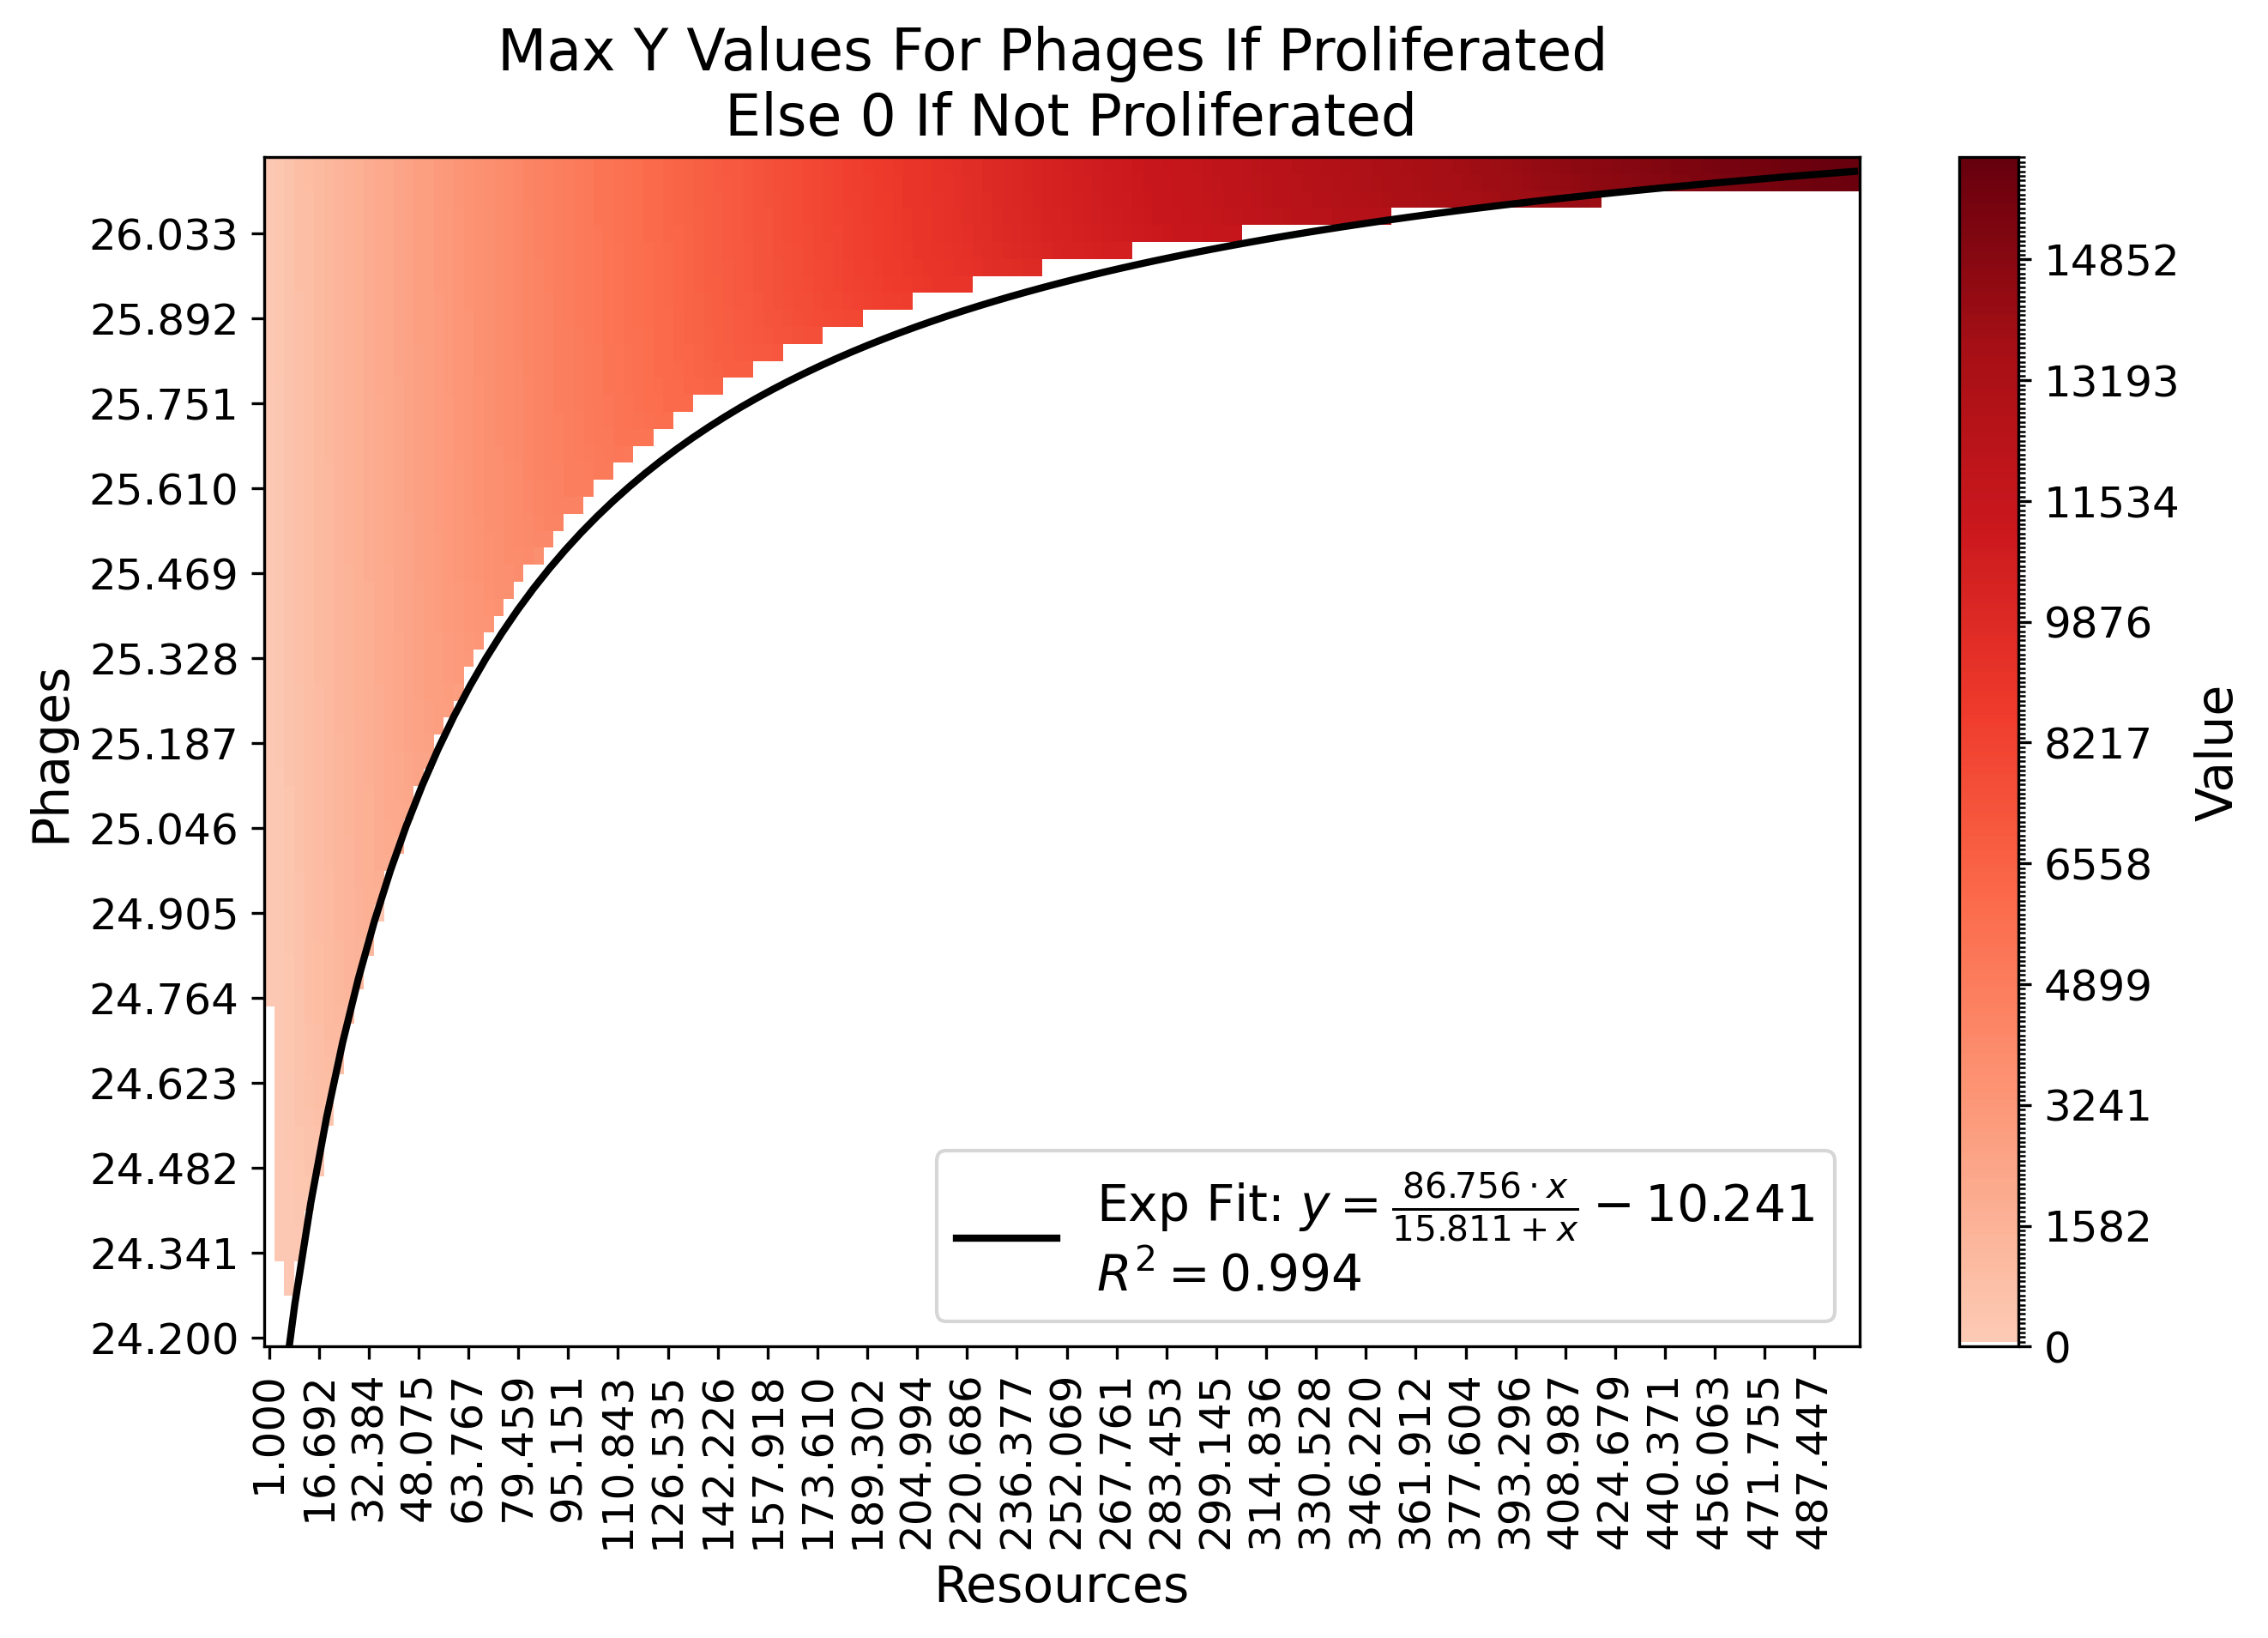
\includegraphics[width=\linewidth]{Plots/Created/PP/phase_portrait_resources_phage.png}
        \caption{
            Phage population proliferation as a function of initial resource and phage concentrations. 
            While the color appears uniform along the vertical axis, each cell is actually a slightly different value. 
            The phage-resource proliferation boundary follows a fitted Monod equation.
        }
        \label{fig:created:phase_portrait_resources_phage}
    \end{subfigure}
    \hfill
    \begin{subfigure}{0.49\linewidth}
        \centering
        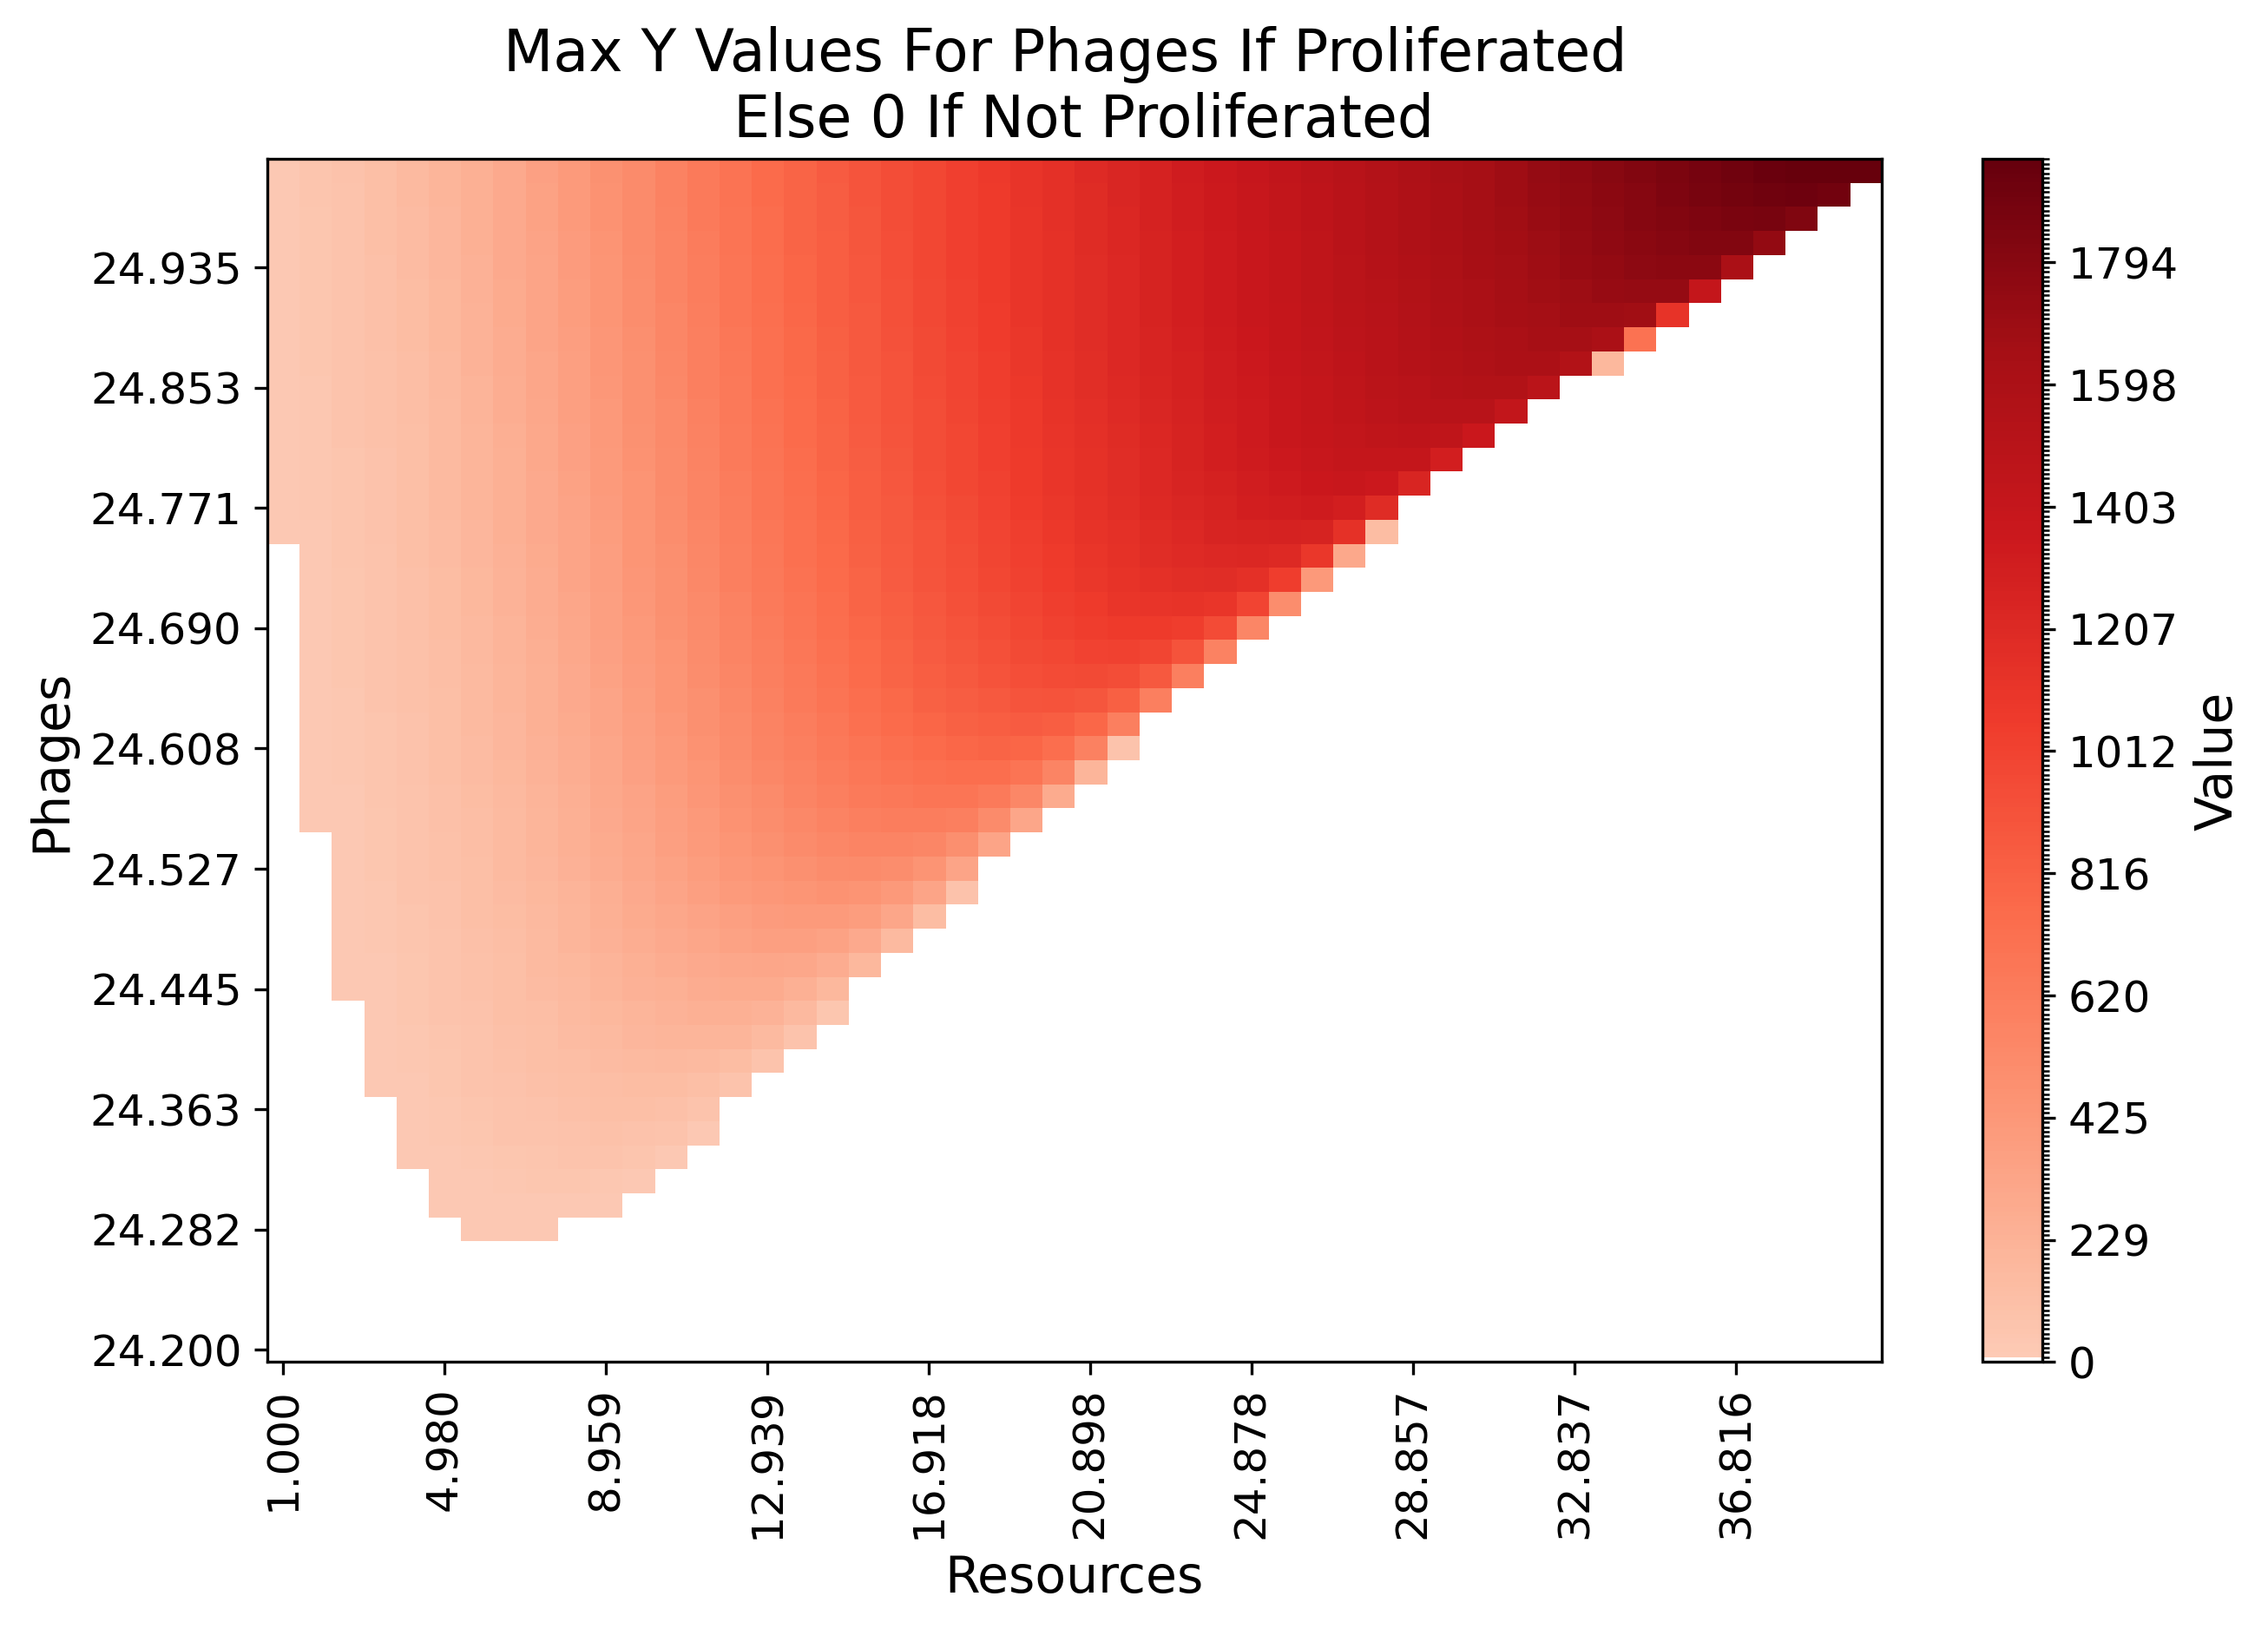
\includegraphics[width=\linewidth]{Plots/Created/PP/phase_portrait_resources_phage_2.png}
        \caption{
            Zoomed in to analyze the regime of behavior change near resources$=10$. 
        }
        \label{fig:created:phase_portrait_resources_phage_2}
    \end{subfigure}
    \caption{
        Varying initial resources and initial phages and the resulting proliferation and fitted proliferation curve. 
        Proliferation is defined as when the phage population reached at least 2 times the initial starting population. 
        This simulation values used can be found in \Cref{tab:appendixE:a_good_curve_2}, but with washout set to 0.02 instead of 0. 
    }
    \label{fig:created:phase_portrait_resource_phage_proliferate}
\end{figure}

\begin{figure}[]
    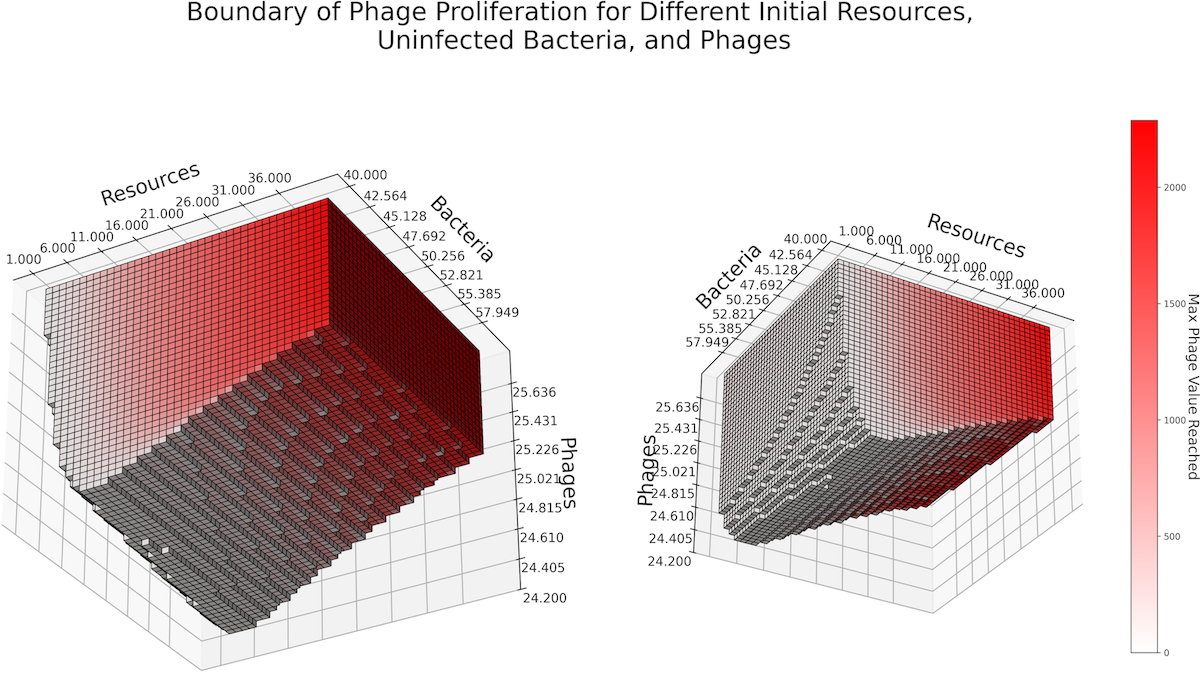
\includegraphics[width=1\textwidth]{Plots/Created/PP/3d_plot_resource_bacteria_phage.png}
    \centering
    \caption{
        3D plot of 
    \label{fig:created:3D_phase_portrait}
    }
\end{figure}

\section{Plotting Parameter Change - $3\times 2\times 3$ Model}
\Cref{fig:created:r_beta_washout_0}, \Cref{fig:created:r_beta_washout_0.02}, and \Cref{fig:created:r_beta_washout_0.05}, show a 7x7 matrix of different $r$ and $\beta$ initial conditions for a $3\times2\times3$ model, and each figure changes the washout rate from 0 to 0.02 to 0.05. 
For each simulation, if $r$ or $\beta$ is equal to a value not equal to $inf$, as identified by the title above each sub-figure, then each value of $r$ or $\beta$ has that value.
All phage initial values started at 10. 
This was specifically chosen to highlight how even though the phage values all start the same, and how two parameter values are controlled, the other parameter values and unequal network topogrpahy has an impact on the population values of the phages. 
If $r$ or $\beta$ is equal to $inf$, then the simulation uses the original data as defined in the IC, vector, and matrix section of the dashboard. 
As a small example for the $3\times 2\times 3$ model, when $r=0.200$, the simulation framework uses $r = \left(\begin{smallmatrix} NaN & 0.200 \\ 0.200 & NaN \\ 0.200 & 0.200 \\ \end{smallmatrix}\right)$ as the input matrix to the ODE model. 
When $r=inf$, the simulation framework uses $r=\left(\begin{smallmatrix} NaN & 0.11695 \\ 0.144459 & NaN \\ 0.11895 & 0.13065 \\ \end{smallmatrix}\right)$ as the data to simulate the interactions with. 
For the cells that don't have an edge between $p$ and $b$ or between $b$ and $r$, the data is represented as $NaN$, short for "Not a Number", \textit{np.NaN}, 

The columns and rows of each figure makes it easy to compare how a change in parameter value affects the curve, while keeping the other parameter the same. 
In $r, \beta, \omega^o=inf, inf, 0$, although not a "good curve" due to limited resource consumption and limited bacterial and phage growth, really shows how the different parameter values for each interaction uniquely affect the growth rate of each agent, especially the phage population (P0=blue, P1=green, and P2=purple). 
Despite all phages starting at the same population level, within the first two or so time units, P1 has less phages than P0 and P2. 
P2 has the fastest initial growth rate, as P2 has the most phages until $t=4$, at which point P1 has a larger phage population. 
P2 reaches its peak population count before P0 or P1, but despite the slower initial growth, P0 and P1 eventually overtake P2 in total phage population. 
P2 also actually reaches its peak before decreasing in population. 
There are trace amounts of infected bacteria at the end of the simulation. 
Since the phage population is reduced by $r_{pb}\cdot(U_b + \sum_{k=1}^M I_{b_k})$, and by specifically choosing the parameter values as used in \Cref{tab:appendixE:complex_model}, behavior that hasn't been seen in a $1\times 1\times 1$ system has been found. 
The complete extinction of the bacteria has been delayed long enough such that at trace amounts, there is phage reduction despite bacteria still existing. 
The peak times for P0, P1, and P2 are $t=6.33, 7.99, 4.52$, a difference of $3.47$ time units. 

Contrast that with the phage population dynamics of that with $r, \beta, \omega^o = inf, 100, 0$, the phage populations do not show interesting dynamics. 
The peak times are more similar and consistent to one another ($t=5.50, 7.01, 6.78$, a difference of $1.51$ time units). 
The phage population curve all appear the same, with slightly slower growth rates. 
There is no crossing of phage populations unlike with $r, \beta, \omega^o=inf, inf, 0$. 

Losing the change in $\beta$ values really affected the dynamics fo the phage population. 
The highlighted example demonstrated the dynamics and influence that multiple agents can have on the final output. 

The top row of \Cref{fig:created:r_beta_washout_0.02} shows how the phages and resources died out relative to the top row of \Cref{fig:created:r_beta_washout_0}. 
Even with a high burst value, the phages could not defeat the pressure from the washout. 
But by changing the $r$ value from $r=0.001$ to $r=0.041$, the phages were able to save themselves and proliferate. 
Using this knowledge, and the information gained from \nameref{sec:results:phase_portrait}, a 3D matrix of phage proliferation can be created. 
\Cref{fig:created:3D_phase_portrait} shows the matrix of proliferation for varying resource, uninfected bacteria, and phage initial conditions. 
The color consistently changes form white to red across the resources axis, and less so across the bacteria or phages axis. 
If spliced along the bacteria axis, there is little difference in the shape of the curve. 
On the underside of the curve, there is some slight variation in color and if the phages proliferated. 
When spliced on the Resource values near 1, there is the decreasing edge of Phage-Bacteria phage proliferation as the initial resource concentration approaches 6. 


\begin{figure}[]
    \centering
    \begin{subfigure}{0.32\linewidth}
        \centering
        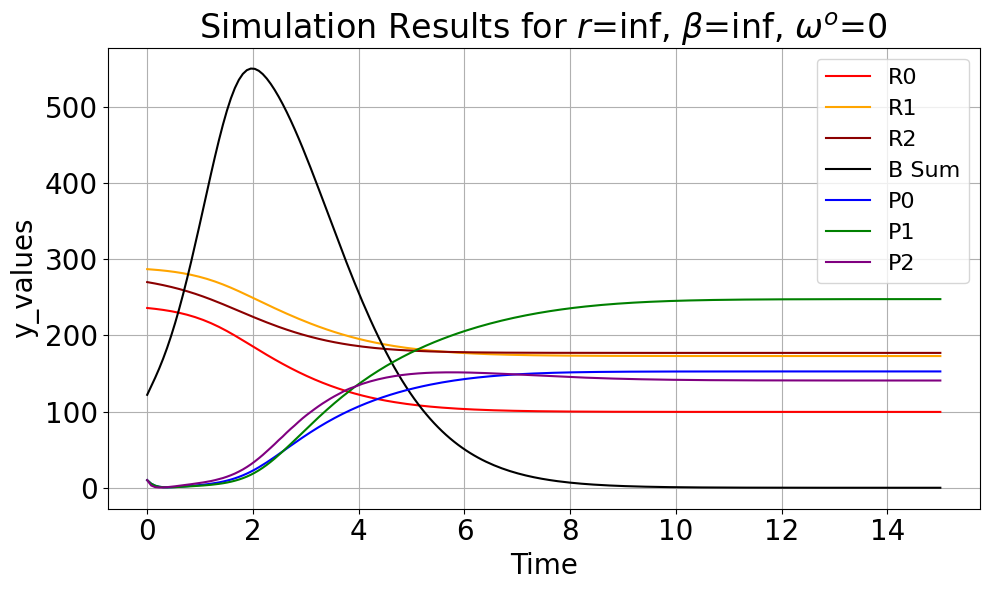
\includegraphics[width=\linewidth]{Images/Plots/Created/UA/r_beta_washout_inf_inf_0.png}
        \caption{
            $r, \beta, \omega^o = inf, inf, 0$, all initial phage condition=10. 
        }
        \label{fig:created:r_beta_washout_inf_inf_0}
    \end{subfigure}
    \begin{subfigure}{0.32\linewidth}
        \centering
        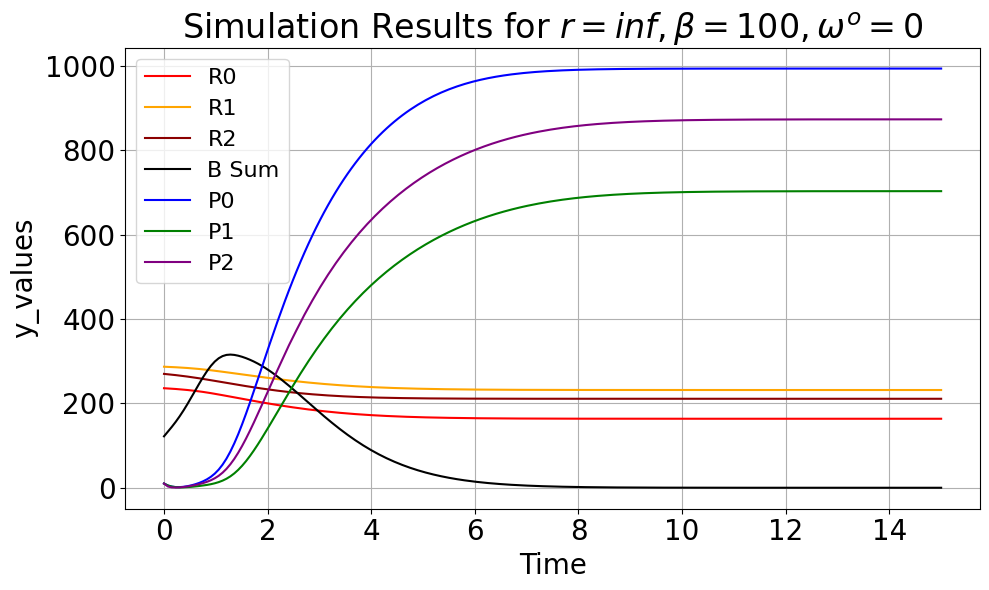
\includegraphics[width=\linewidth]{Images/Plots/Created/UA/r_beta_washout_inf_100_0.png}
        \caption{
            $r, \beta, \omega^o = inf, 100, 0$, all initial phage condition=10. 
        }
        \label{fig:created:r_beta_washout_inf_100_0}
    \end{subfigure}
    \begin{subfigure}{0.32\linewidth}
        \centering
        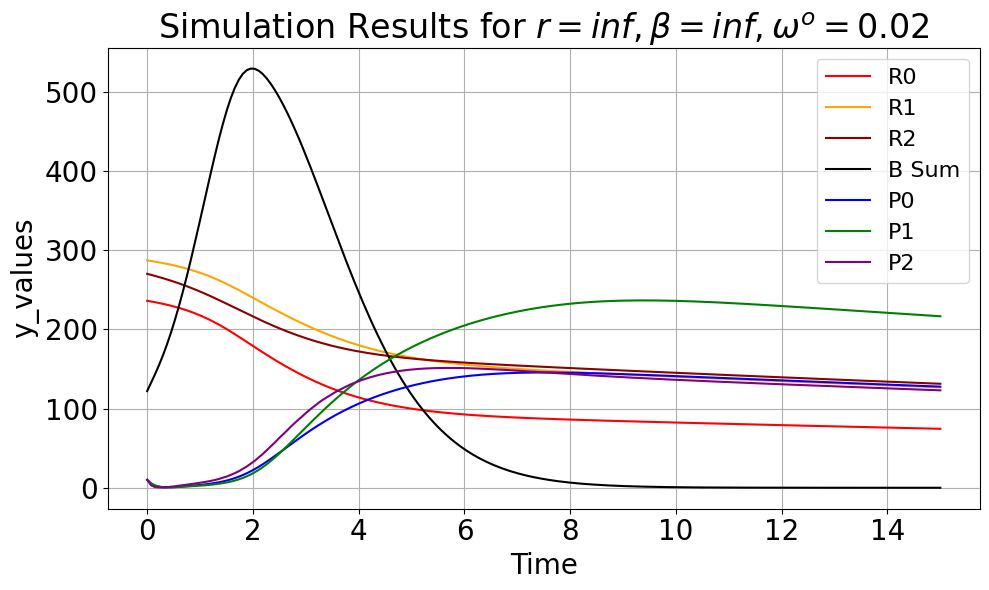
\includegraphics[width=\linewidth]{Images/Plots/Created/UA/r_beta_washout_inf_inf_0.02.png}
        \caption{
            $r, \beta, \omega^o = inf, inf, 0.02$, all initial phage condition=10. 
        }
        \label{fig:created:r_beta_washout_inf_inf_0.02}
    \end{subfigure}
    \caption{
        Varying $r$, $\beta$, and $\omega^o$. 
        All phage values set to 10 to show how the network connections and vector/matrix values affect phage growth. 
        Selectively chosen sub-figures from \Cref{fig:created:r_beta_washout_0}, \Cref{fig:created:r_beta_washout_0.02}, and \Cref{fig:created:r_beta_washout_0.05}. 
        Chosen parameter values can be found in \Cref{tab:appendixE:complex_model}. 
    }
\end{figure}

\section{Phage, Bacteria, and Resource Survivability For a $20\times20\times10$ System}
Finally a large $20\times20\times10$ system can be created